%----------------------------------------------------------------------------------------
% Introduction
%----------------------------------------------------------------------------------------
\setcounter{page}{1} % Sets counter of page to 1

\section{Introduction} % Add a section title

\subsection{Importance of Cross-Chain Interoperability in Blockchain} 

In the early days of the Internet, on-line systems were fragmented. Different networks operated in isolation, each with its proprietary protocols, making it difficult for users to access and exchange information seamlessly. This fragmented approach stifled innovation and limited the potential of the Internet. The advent of the World Wide Web, with its standard protocols like HTTP and TCP/IP, transformed this landscape by enabling universal connectivity~\cite{www}. It created a unified, interoperable platform that revolutionized global communication, commerce, and collaboration. Similarly, blockchain technology today faces a comparable challenge: Thousands of independent blockchains operate as siloed ecosystems, each with its own protocols, standards, and functionality.

Cross-chain operability is the blockchain equivalent of the standardization brought about by the World Wide Web. By allowing different blockchain networks to communicate and interact seamlessly, it unlocks the full potential of decentralized technologies. Users can transfer assets, share data, and execute smart contracts across multiple chains without having to navigate the technical and logistical complexities of each. This interoperability fosters innovation by allowing developers to build decentralized applications (dApps) that leverage the strengths of multiple chains, be it scalability, security, or cost efficiency. It ensures that the blockchain ecosystem evolves as a cohesive, interconnected network, much like how the internet evolved into a global information superhighway.

As discussed in~\cite{crosschain}, one of the main challenges is the heterogeneity of blockchain platforms. Each blockchain operates with its own protocols, consensus mechanisms, and data structures, creating significant barriers to seamless interaction. This diversity leads to "disconnected value islands," where assets and data are confined within individual blockchains, limiting their utility and the broader potential of blockchain technology. Another critical issue is the security vulnerabilities inherent in cross-chain interactions. In~\cite{crosschain}, Harris, C. G. discusses various exploits and attacks that have targeted cross-chain bridges and interoperability protocols, underscoring the need for robust security measures. Ensuring the integrity and authenticity of transactions across different blockchains remains a formidable challenge. 

Despite these challenges, the article describes several opportunities to improve blockchain interoperability. The development and implementation of standardized protocols can facilitate more straightforward communication between disparate blockchains. By establishing common standards, interoperability solutions can be more easily adopted, promoting a more cohesive blockchain ecosystem~\cite{mao}. Furthermore, cross-chain technologies have high potential to foster innovation in decentralized applications (dApps). By enabling dApps to operate across multiple blockchains, developers can leverage the unique features and capabilities of different platforms, leading to more versatile and powerful applications. This cross-chain functionality can drive the next wave of growth and adoption in the blockchain space. 

\begin{figure}[h!]
    \centering
    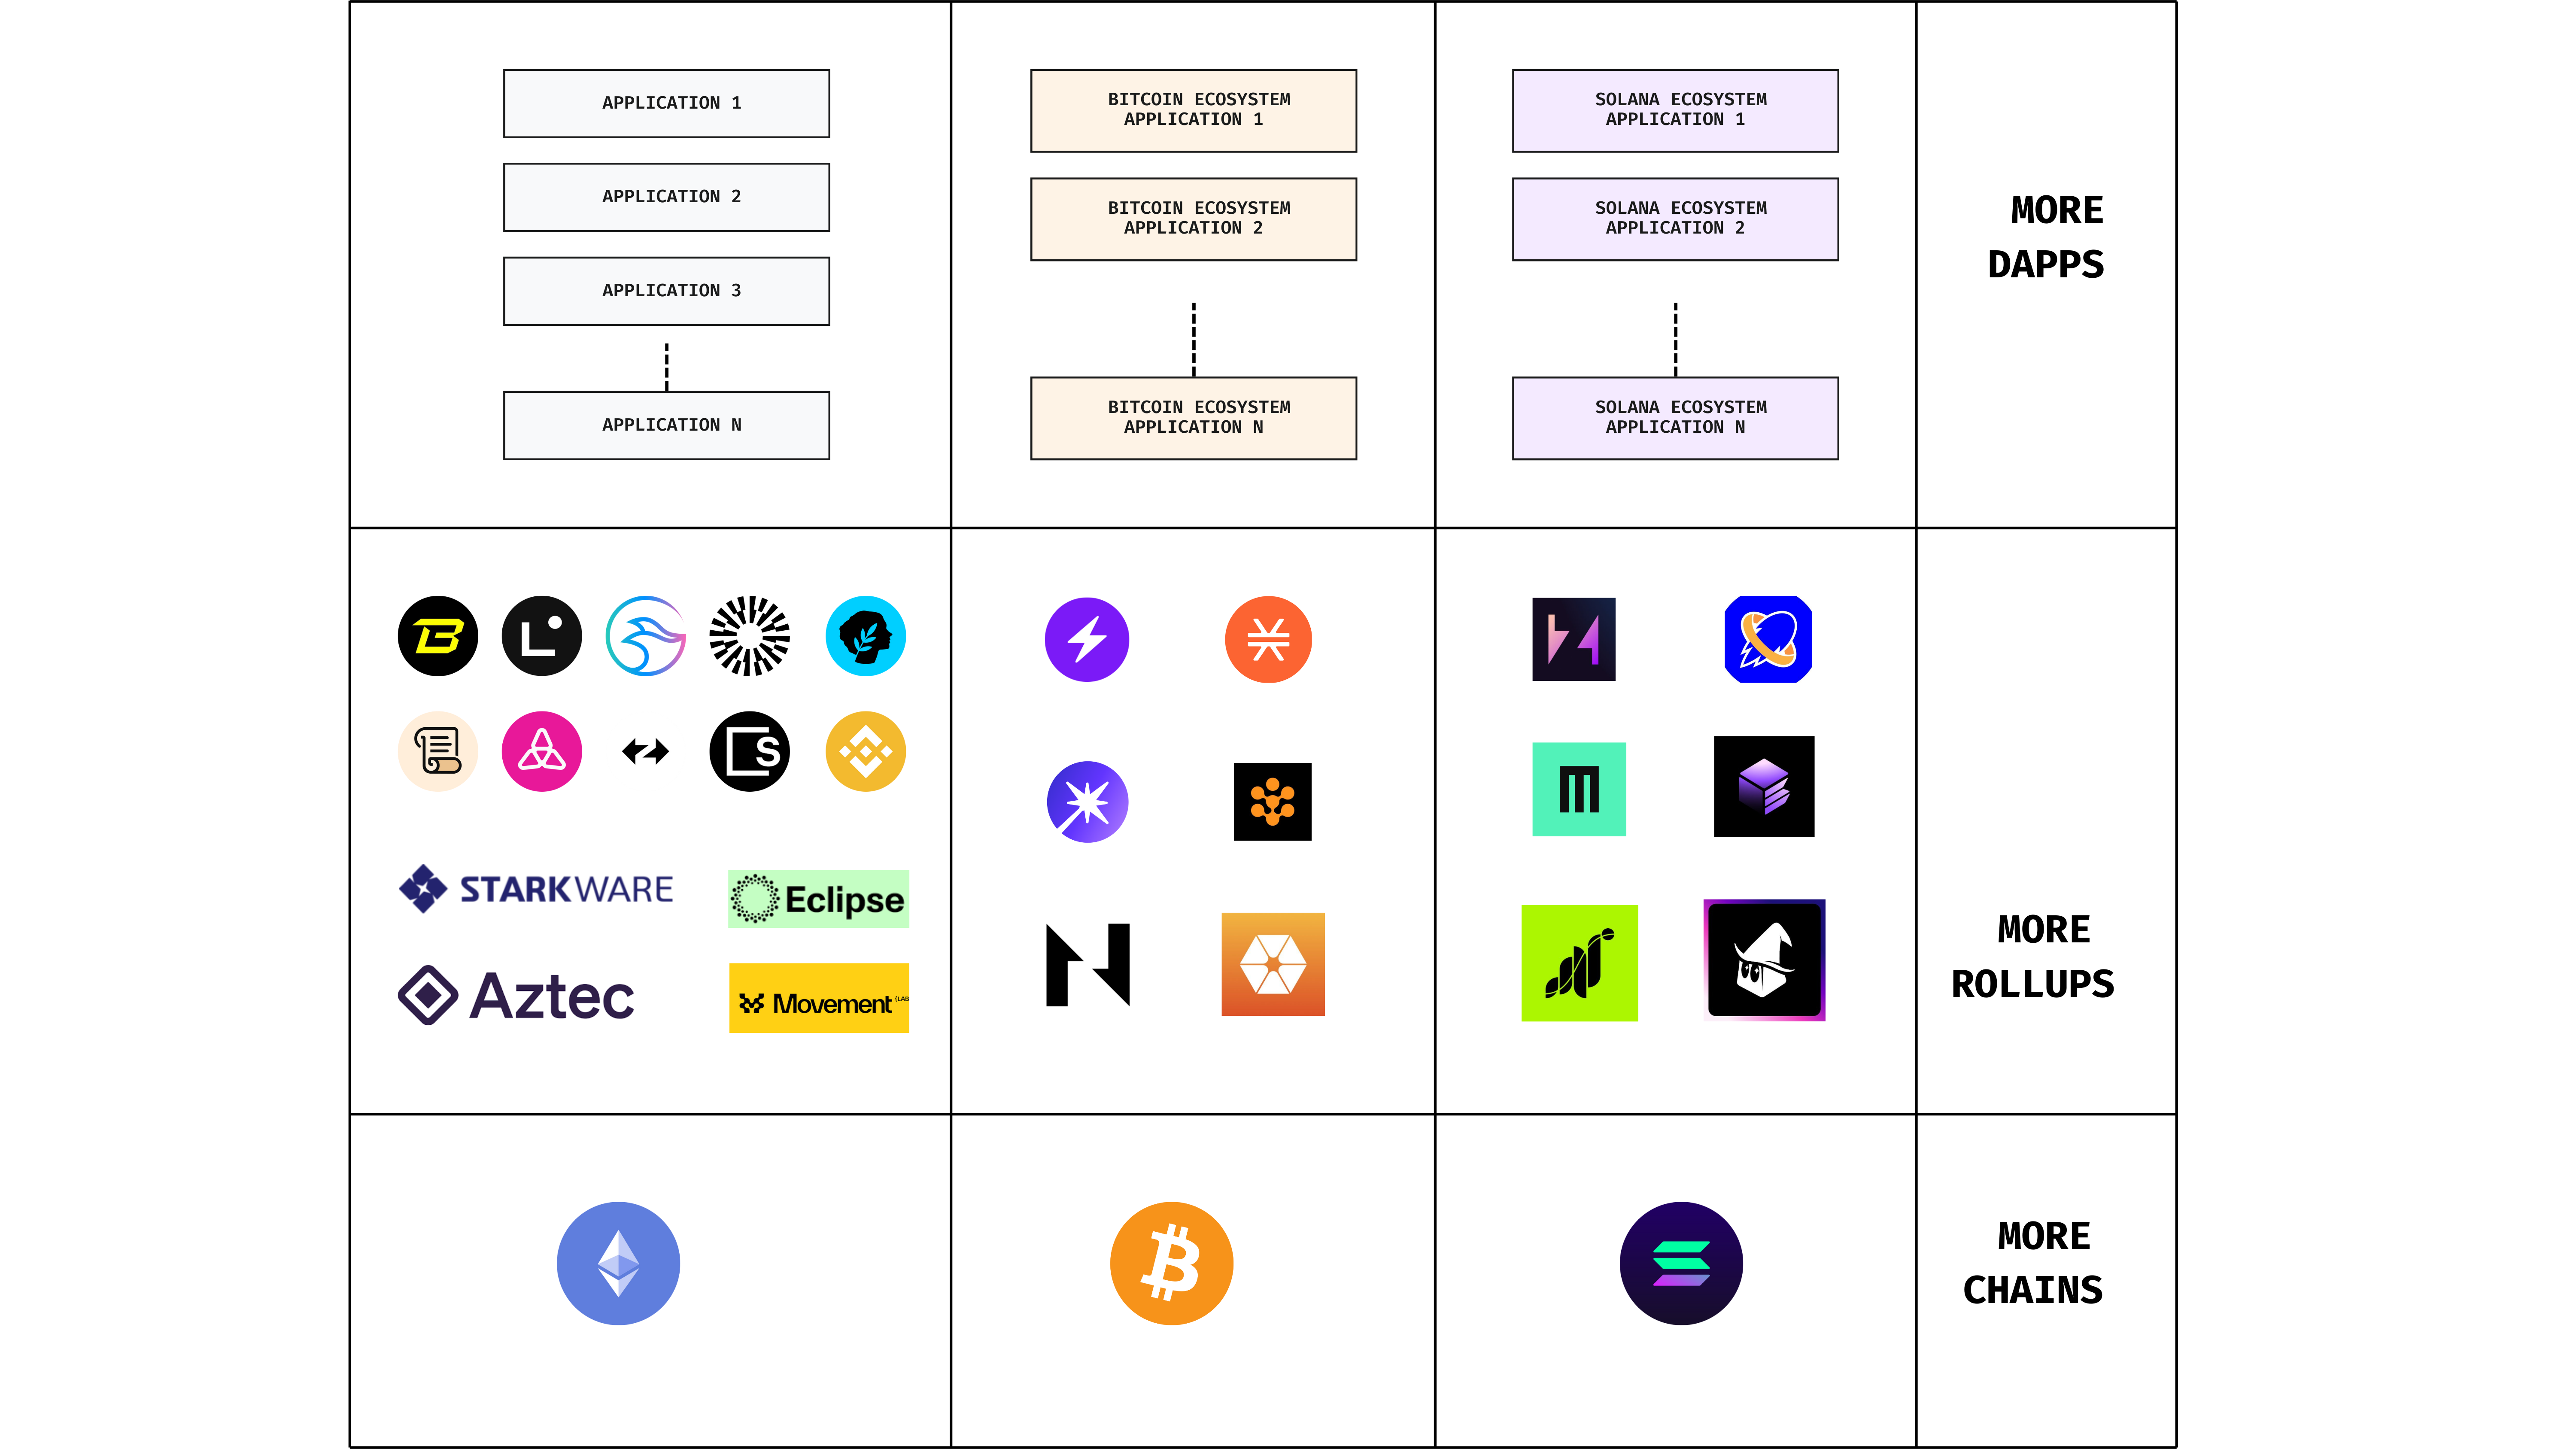
\includegraphics[width=0.99\linewidth]{figure/fragmented.png}
    \caption{Fragmented Ecosystem}
    \label{fig:fragmented}
\end{figure}


\subsection{Existing approaches}

The cross-chain ecosystem is rapidly evolving, with various solutions addressing the need for interoperability between blockchains at different layers of the stack. These solutions can generally be categorized into three key types~\cite{particle}:

1. Foundational solutions: These provide the underlying infrastructure and protocols necessary for cross-chain communication. They focus on enabling basic interoperability between chains and offering a solid foundation on which other solutions can be built.

2. Mid-level solutions: These solutions manage and coordinate cross-chain transactions and interactions. They abstract away the complexities of interoperability for decentralized applications (dApps) and ensure that data and assets can flow smoothly across different chains.

3. Comprehensive solutions: These full-stack solutions aim to cover all aspects of cross-chain interoperability, including communication, liquidity, and more. They offer broader compatibility across ecosystems and address multiple layers of interoperability in a single package. 

Each category serves a specific role in ensuring seamless communication and asset transfers between different blockchain ecosystems. However, challenges such as fragmentation and dependency bottlenecks persist, as protocols at one level depend on those beneath them. Let’s explore the existing solutions at these levels, detailing their focus areas and limitations.

\subsubsection{Foundational Solutions}

Foundational solutions focus on providing the underlying infrastructure and protocols to support cross-chain interactions. These solutions offer the base upon which other systems can build interoperability.

\textbf{LayerZero}: LayerZero~\cite{layerzero} is a protocol designed for seamless communication between heterogeneous blockchains. Specifically, it focuses on providing a universal messaging layer that can interconnect chains without restricting the system to a specific blockchain or ecosystem. Using a modular approach, LayerZero ensures that it can connect to various chains at different levels, providing a robust foundation for decentralized applications (dApps) and other protocols. The core strength of the protocol lies in its ability to facilitate trustless cross-chain messaging with minimal reliance on intermediary chains. Although LayerZero provides foundational interoperability, it still requires third-party oracles and relayers, introducing some degree of trust and centralization risk. Additionally, it does not provide solutions for handling fragmentation across ecosystems like Ethereum, Polygon, and others.

\textbf{Axelar Network:} Axelar~\cite{axelar} offers cross-chain messaging solutions that connect different blockchains in a decentralized manner. The network uses a unique approach to ensure that cross-chain transactions are routed securely, making it easier for dApps to interact across ecosystems without worrying about the underlying complexities. The key focus of Axelar is to provide a simple and unified solution that ensures a seamless experience for developers and users alike. Although Axelar supports several blockchains, its focus has been primarily on bridging Ethereum and Cosmos ecosystems, limiting the scope in terms of interoperability with other non-Cosmos- or Ethereum-based chains. Furthermore, Axelar faces scalability challenges, as it scales to support a wider variety of chains.

\textbf{Thorchain:} Thorchain~\cite{thorchain} is a decentralized liquidity protocol designed to allow cross-chain asset swaps. By using an innovative mechanism that does not rely on wrapped tokens, Thorchain enables native asset swaps between chains. Its focus on liquidity makes it particularly useful for decentralized finance (DeFi) applications. Thorchain’s reliance on native asset swaps could lead to scalability challenges, especially as it grows to support more chains. Its ecosystem is also largely focused on DeFi, limiting its applicability in broader cross-chain use cases.


\subsubsection{Mid-level Solutions}

Mid-level solutions facilitate the coordination and management of cross-chain transactions and interactions. These solutions typically abstract away the complexities of cross-chain operations for dApps and users.

\textbf{Agoric}: The focus of Agoric~\cite{agoric} is on enabling smart contracts for the creation of decentralized applications that can span multiple blockchains. Agoric brings together both foundational solutions and mod-level through its JavaScript-based environment for smart contract execution, targeting DeFi applications and cross-chain interoperability. It allows developers to create multi-chain smart contracts, but it still faces limitations with chains outside of the EVM ecosystem.

\textbf{Socket}: Socket~\cite{socket} is a cross-chain communication platform built for DeFi applications, enabling seamless communication across different blockchain networks. The main feature of the socket is its ability to support decentralized applications and services running on different L1 and L2 networks. However, its ecosystem is still somewhat Ethereum-centric and could face challenges as more non-Ethereum ecosystems like Move gain momentum.

\textbf{Skip}: Skip~\cite{skip} is a cross-chain protocol that simplifies the process of enabling decentralized applications to communicate across chains. Its focus is on supporting token and data transfers with minimal latency. Skip’s ability to work with both Ethereum-based and non-Ethereum chains makes it a promising option, but scaling to accommodate a wider range of L1 and L2 chains remains a key challenge.

\subsubsection{Comprehensive Solutions}

Comprehensive solutions are full-stack solutions designed to cover all aspects of cross-chain interoperability, including communication, liquidity, and more, while offering more extensive compatibility across ecosystems.

\textbf{Arbitrum}: Arbitrum~\cite{arbitrum} is a Layer 2 scaling solution for Ethereum that leverages optimistic rollups to improve scalability and transaction throughput. While it is primarily focused on enhancing Ethereum's scalability, it has opened up a pathway for supporting Ethereum-compatible chains and applications, making it an important player in the broader Layer 2 ecosystem. Arbitrum's focus on Ethereum means that it is limited in its ability to facilitate cross-chain interoperability outside of the Ethereum ecosystem. Furthermore, with multiple rollups being developed for Ethereum, fragmentation within the Ethereum ecosystem could increase as more L2 solutions are deployed, each with their own interoperability protocols and standards.

\textbf{Omni Network}: Omni Network~\cite{omni} offers cross-chain interoperability solutions at the Layer 2 level. It provides interoperability for various rollups and Layer 2 chains built on Ethereum. By using a robust messaging protocol, Omni Network can facilitate seamless interaction between different Ethereum-based Layer 2 solutions. Like many other Ethereum-centric solutions, Omni Network's focus remains limited to Ethereum-based ecosystems. As Ethereum rollups proliferate, the fragmentation of standards and protocols will complicate cross-chain interactions even further. Additionally, Omni's solution does not address interoperability with other Layer 1 ecosystems or new emerging ecosystems like Move-based networks.

\textbf{Polygon’s AggLayer}: Polygon’s AggLayer~\cite{aggglayer} offers an L2 scaling solution with enhanced cross-chain interoperability. It aims to improve transaction throughput across various blockchains by creating aggregated layers for data and transaction processing. Despite its innovative nature, the solution still faces the challenge of dealing with interoperability between various non-Ethereum chains, especially with the growth of Move-based rollups and L2s.

\textbf{NEAR}: NEAR Protocol~\cite{near} is designed to facilitate scalability and ease of use with a strong focus on user experience. It provides cross-chain interoperability through its bridge solutions, enabling it to communicate with Ethereum and other networks. While NEAR’s ecosystem is expanding, the continued growth of non-Ethereum chains and new smart contract languages like Move pose a challenge to its scalability and interoperability in the long term.

\textbf{Optimism’s Superchain}: Optimism’s Superchain~\cite{optimisim} focuses on interoperability at the L2 level, using the Optimistic Rollup architecture to enable Ethereum scalability. The Superchain approach envisions a multichain ecosystem powered by Optimism’s scaling technology, but its reliance on Ethereum could limit its cross-chain capabilities as other ecosystems, such as Move, develop and emerge with different architectures and priorities.

\subsubsection{Bottlenecks and Dependencies Across Layers}

One of the key challenges facing the development of cross-chain interoperability is the bottleneck effect that arises from the dependency between different protocol layers. The foundational protocols rely on the security and performance of the chains they are connected to. For example, if a foundational solution like LayerZero or Axelar faces issues in communication or scalability, it could cause disruptions for higher-level  solutions like Agoric or Socket, which, in turn, would impact the overall user experience and reliability of comprehensive solutions like Polygon’s AggLayer or Arbitrum.

As each level is co-dependent on the one below, the compromise of a protocol at the foundational layer can cause cascading failures or reduced functionality across all other layers. To address this challenge, a comprehensive solution would need to work with multiple foundational protocols while mitigating the risks of fragmentation and ensuring strong cross-chain communication across all levels.

In summary, the landscape of cross-chain interoperability solutions is diverse, with foundational, mid-level, and comprehensive solutions offering different levels of integration. However, with the emergence of new ecosystems and the rise of Move-based rollups, it is clear that the industry must adapt to these changes or face further fragmentation and siloing across the blockchain space.

\subsection{Overview of the Omnichain Web} % Add a subsection

Omnichain Web stands out as a truly comprehensive solution by offering a unified framework for seamless interoperability across all blockchains, bypassing the bottlenecks that traditional solutions face. Unlike existing comprehensive solutions, which are often constrained by their reliance on specific ecosystems or foundational protocols, Omnichain Web integrates multiple L1s, L2s, and even emerging ecosystems like Move, enabling decentralized applications (dApps) to operate across the entire blockchain landscape without friction. By abstracting away the complexity of cross-chain interactions and providing a robust layer of universal communication, Omnichain Web eliminates the cascading failures that occur when one layer encounters issues. This holistic approach ensures that the infrastructure remains secure, scalable, and future-proof, allowing developers to focus on innovation without worrying about fragmentation or dependency on a single ecosystem. With Omnichain Web, blockchain interoperability is no longer a challenge but a seamless and reliable experience for both developers and users alike.

\begin{figure}[h]
    \centering
    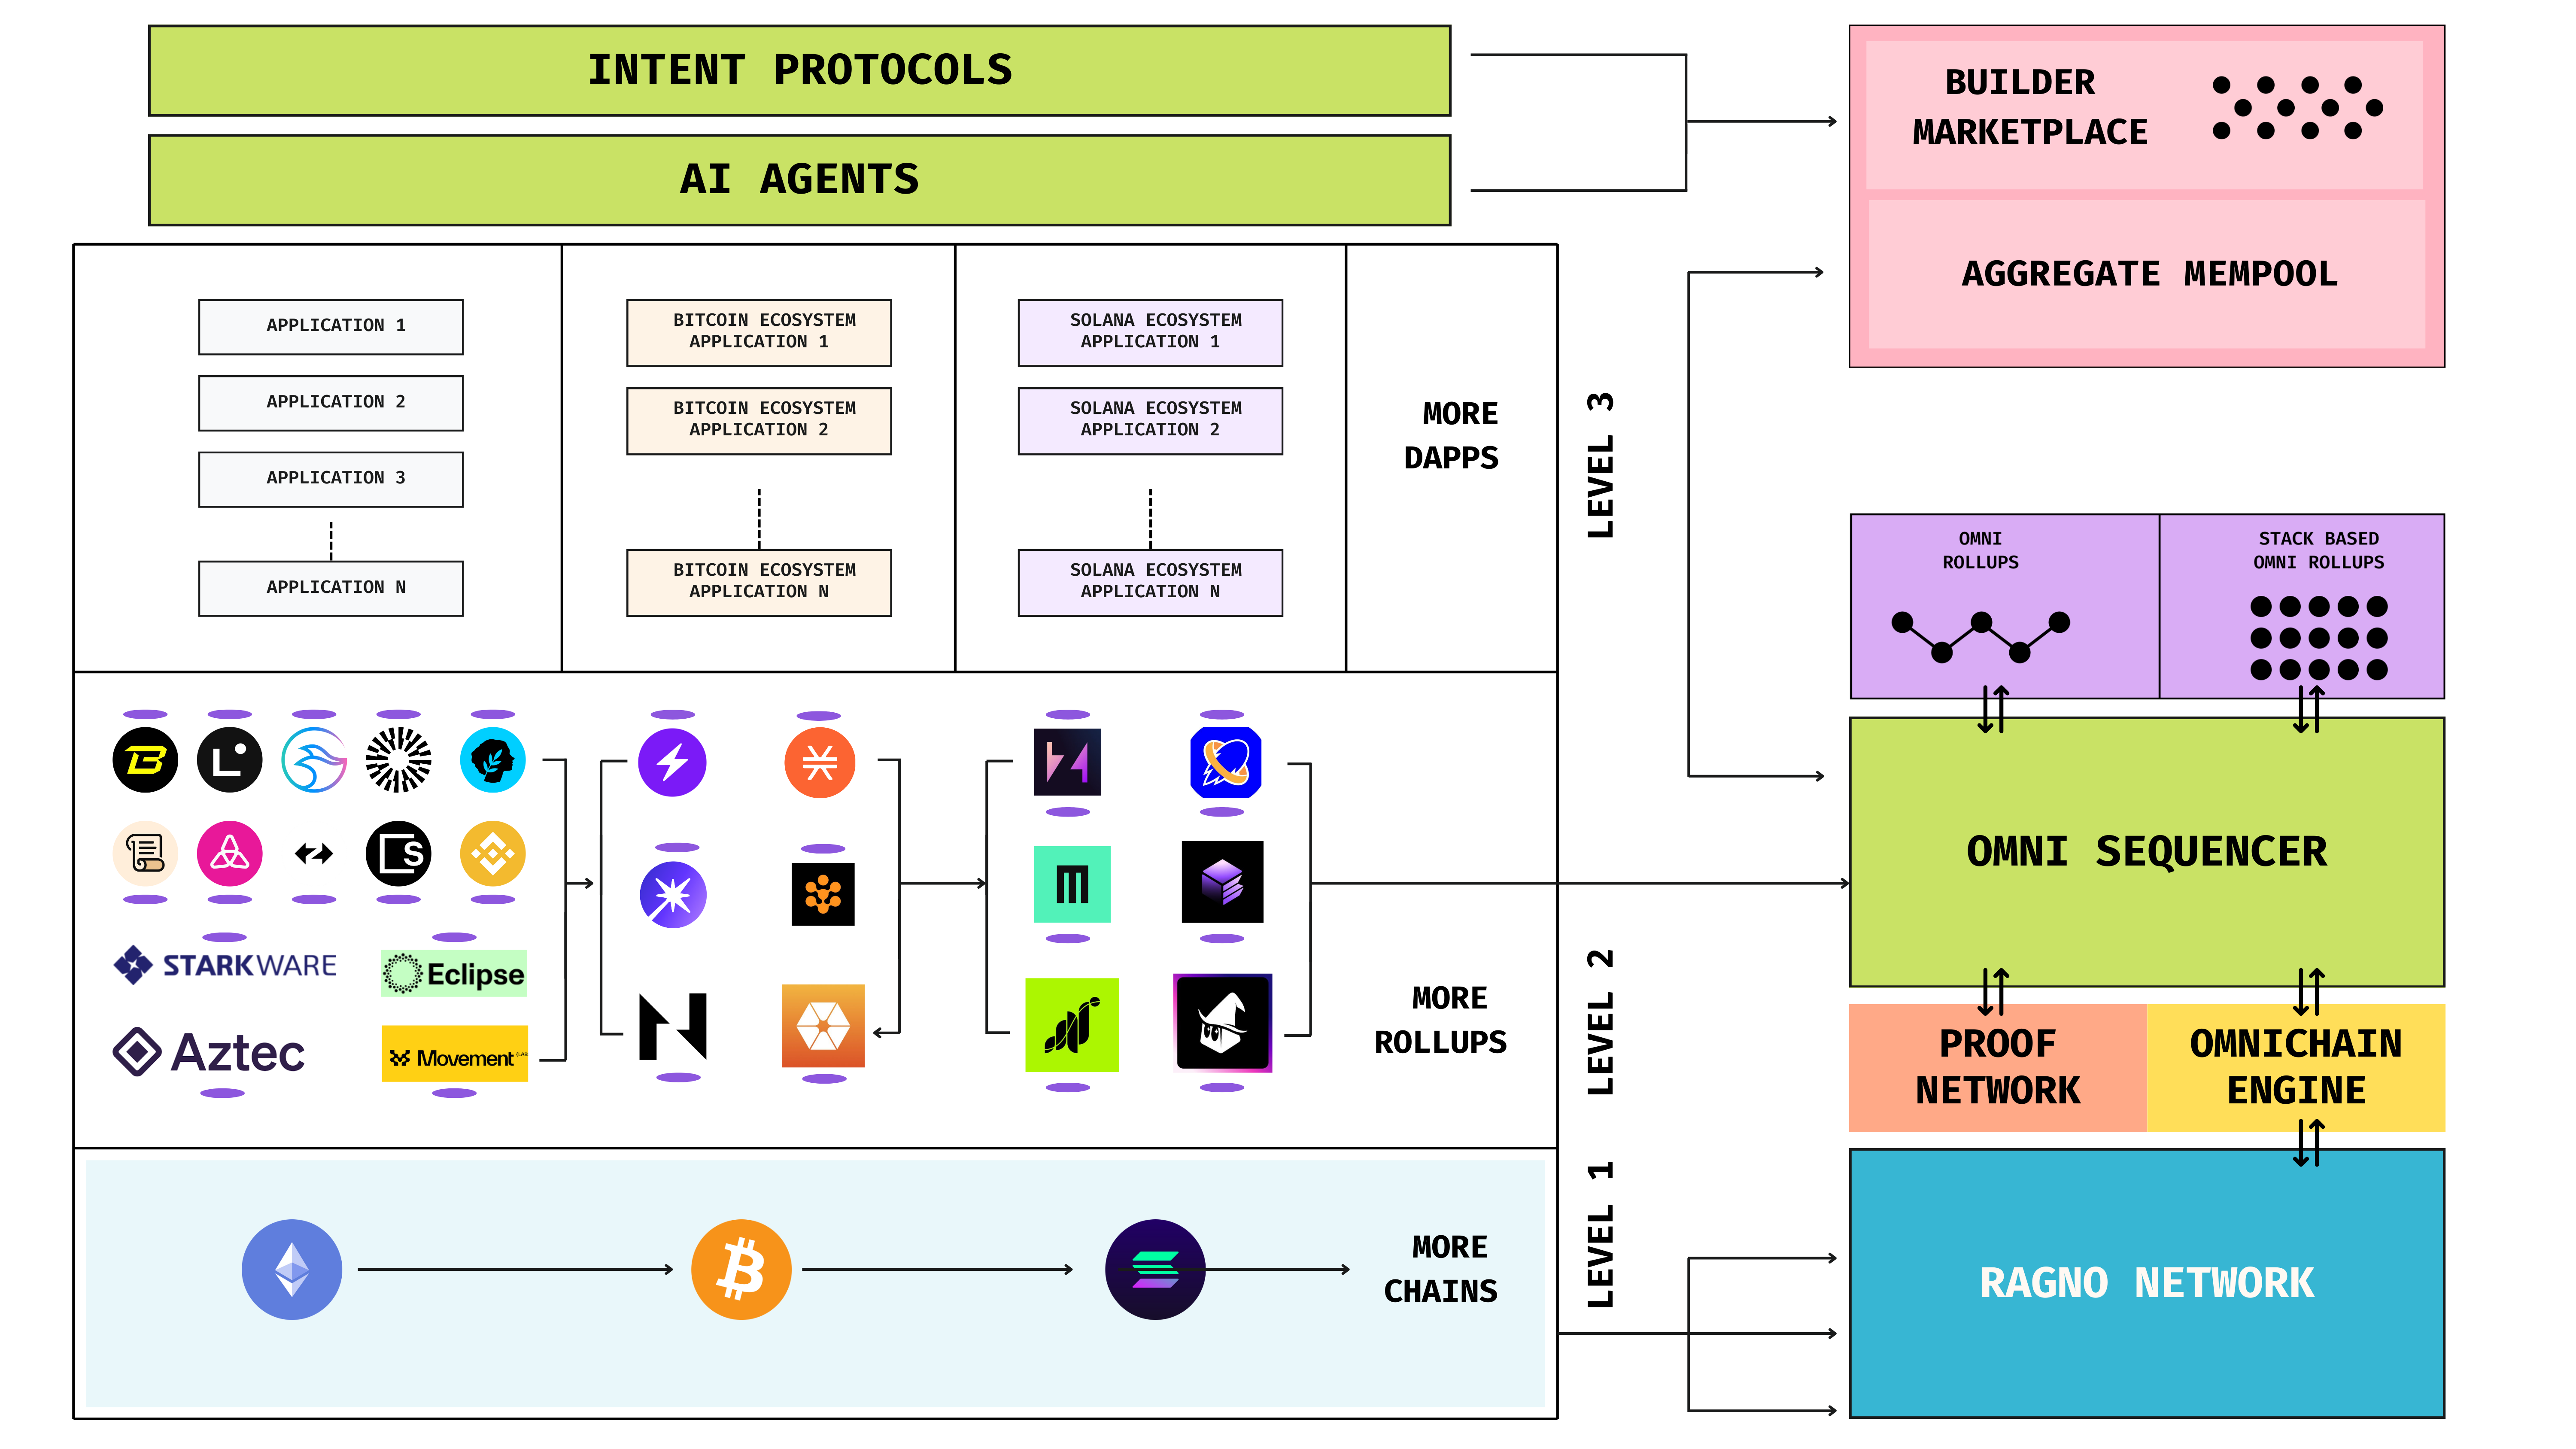
\includegraphics[width=0.99\linewidth]{figure/connected.png}
    \caption{Connected Ecosystem}
    \label{fig:connected}
\end{figure}

The Omnichain Web consists of four core components: Builder Marketplace, Omni Sequencer, Prover Network, and Ragno Network. Each part plays a distinct role in ensuring efficient, secure, and interoperable operations across the ecosystem.

\begin{itemize}
    \item[1.] \textbf{Builder Marketplace}

%The Builder Marketplace serves as the ecosystem's application layer, hosting decentralized applications (dApps) and solvers that are deployed in Trusted Execution Environments (TEE) for enhanced integrity and security.

The Builder Marketplace is responsible for unifying protocols from all chains into structured modules, enabling developers to build customized solvers with cross-communication capabilities. It supports universal transaction flows from intent-centric apps, AI agents, and direct API calls, ensuring seamless interoperability and efficiency.

Features:
    \begin{itemize}
        \item Applications such as AI Agent and Intent Protocol enable users to submit inputs for processing.
        \item Users can interact with solvers through multiple interfaces, such as customized frontends, AI agents, TEE environments, or by directly utilizing solver API endpoints.
        \item Solvers process inputs and produce optimized transaction batches for further processing.
    \end{itemize}

    \item[2.] \textbf{Omni Sequencer}

The Omni Sequencer is responsible for aggregating and organizing transactions from solvers, rollups, or direct user submissions.

Functionality:
    \begin{itemize}
        \item Receives transactions via a sequencer client and bundles them into blocks based on settlement chains.
        \item Orders transactions and generates commitments to the ordering.
        \item Publishes commitments to a Data Availability (DA) layer or smart contract.
        \item Sends blocks to the rollup executor for execution and settlement.
    \end{itemize}
    

    \item[3.] \textbf{Prover Network}

The Prover Network underpins the ecosystem’s cryptographic security by providing proofs for state transition functions.

Key Features:
    \begin{itemize}
        \item Distributed Jolt-based zkVM for generating computational proofs.
        \item Utilizes the Binius proof system, optimized for binary operations critical to machine computations.
        \item Generates proofs for rollup state transitions, ensuring the validity of updates before they are sent to settlement chain contracts.
    \end{itemize}
    

    \item[4.] \textbf{Ragno Network}

The Ragno Network ensures robust data aggregation and transaction validation through its operators and Hermes Chain. The settlement process involves pre-confirmation on the Hermes Chain and verification of source chain execution before finalizing on the target chain.

Components:
    \begin{itemize}
        \item Operators: Nodes registered on the Hermes chain, responsible for fetching and processing blocks from different chains.
        \item Crawler: Maintains an updated list of operators and filters blocks for transactions related to Dojima Chain.
        \item Hermes: Publishes filtered transactions on the Hermes Chain and processes them.
        \item Narada: Signs outbound transactions using GG20 TSS and passes them to the respective rollup for execution, with additional verification by the Crawler. 
    \end{itemize}
    
\end{itemize} 